\hypertarget{section-introduction-and-goals}{%
\section{Project-Vision and Goals}\label{section:introduction-and-goals}}

The Escape Doom system aims to provide FH Campus Wien with a platform for creating educational escape rooms. In the first semester of our Bachelor’s program, we participated in a programming escape room that offered an engaging, interactive learning experience. Inspired by this positive experience, we want to create a platform that allows students to easily access and play similar escape rooms.


\subsection{Motivation}

Initially, instructors of FH Campus Wien manually created and managed escape rooms by coding each one from scratch. This approach allows for unique, tailored experiences, but it is labor-intensive and difficult to maintain over time, especially as riddles need to be refreshed every one to two years to prevent sharing of solutions between cohorts. This inspired us to develop our own version of an escape room to explore the potential for creating a scalable, reusable platform.

In the current situation, our project—while functional—still requires participants to use an IDE (with the code accessible) which limits usability and makes solutions to code-based challenges more easily discoverable. Our goal is to address these limitations by transforming the project into a streamlined, maintainable system—or in other words, a product—that reinforces the educational value of the escape room.

\subsection{Product Vision}

Our target groups include both students and instructors at FH Campus Wien. For students, we aim to create an escape room platform that enhances learning by providing a fun, interactive environment with near real-time collaboration and an intuitive, browser-based coding experience. For instructors, we aim to provide a maintainable system that allows them to use escape rooms as an educational tool, with the future goal of enabling them to design and configure their own escape rooms.

Our vision is to develop a tool that enables instructors to create and manage user-friendly and accessible point-and-click escape rooms for their courses, with functionality similar to CodinGame escape rooms.\footnote{\url{https://escape.codingame.com/}}



\begin{figure}[h!]
    \centering
    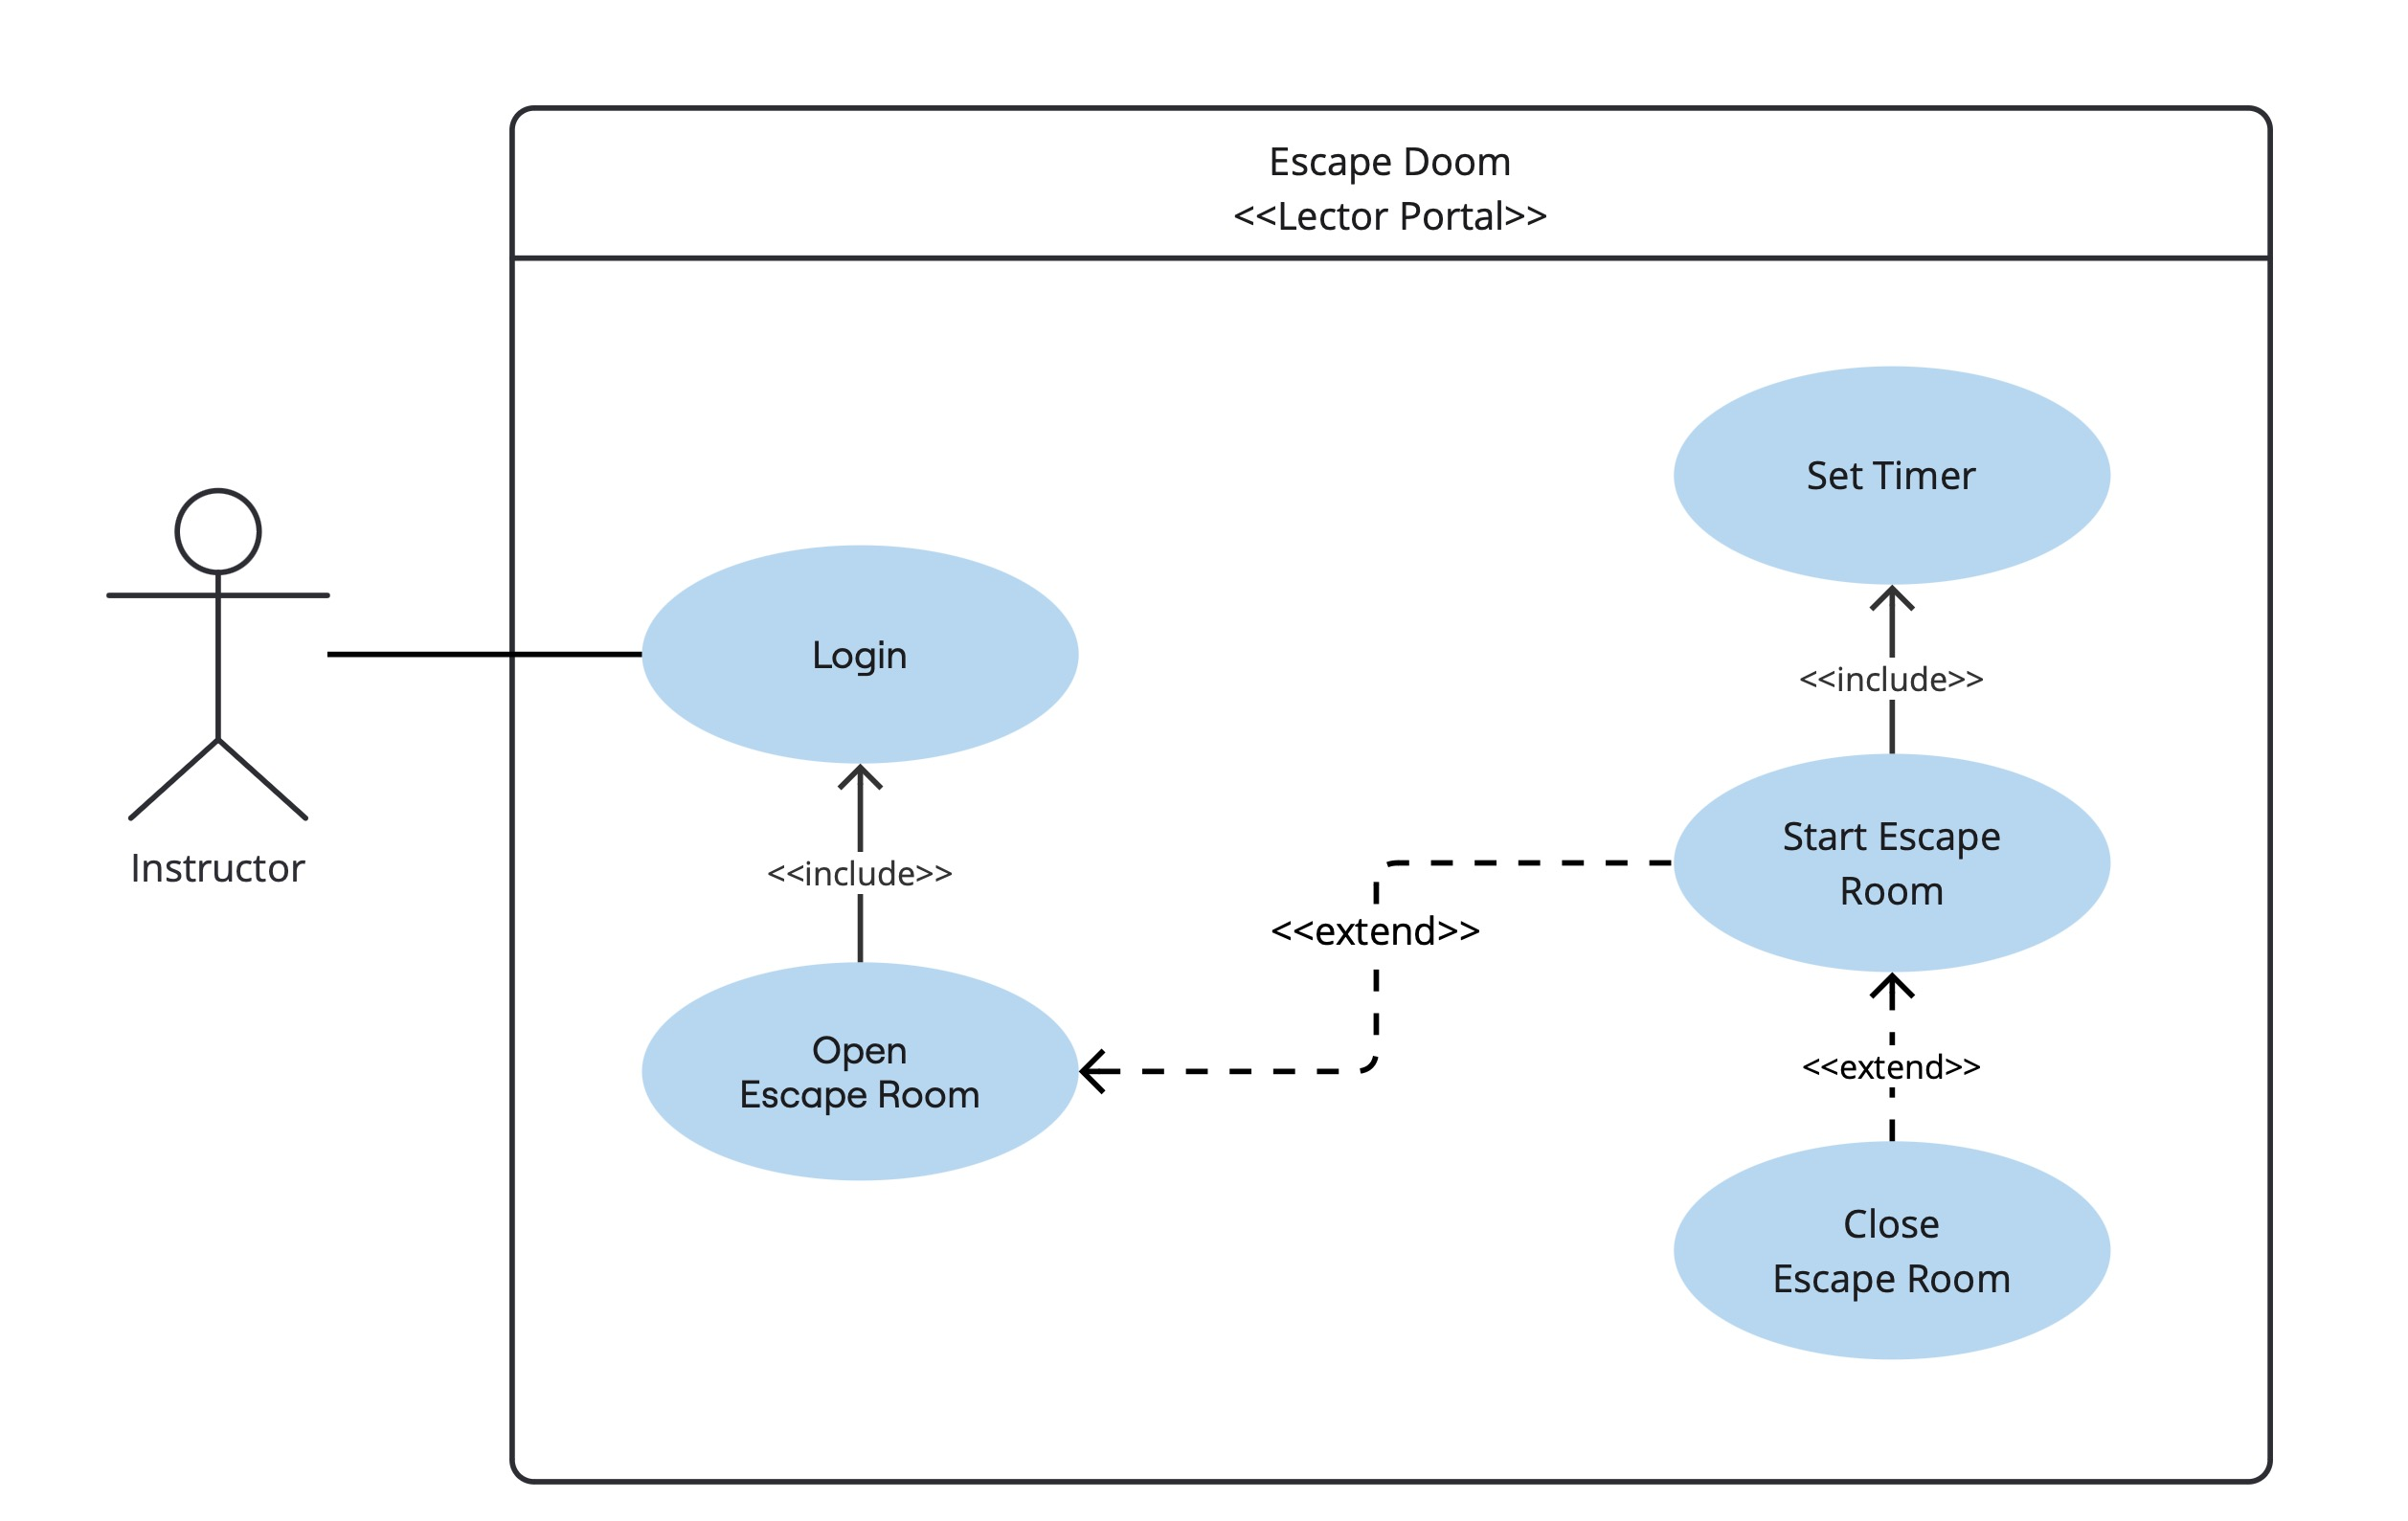
\includegraphics[width=\linewidth]{UC-01.png}
    \caption{UC01 - Lector Portal}
    \label{fig:uc-01}
\end{figure}



\begin{figure}[h!]
    \centering
    \includegraphics[width=\linewidth]{images/LectorPortal.png}
    \caption{Lector Portal Mockup}
    \label{fig:lector:portal}
\end{figure}


\begin{figure}[h!]
    \centering
    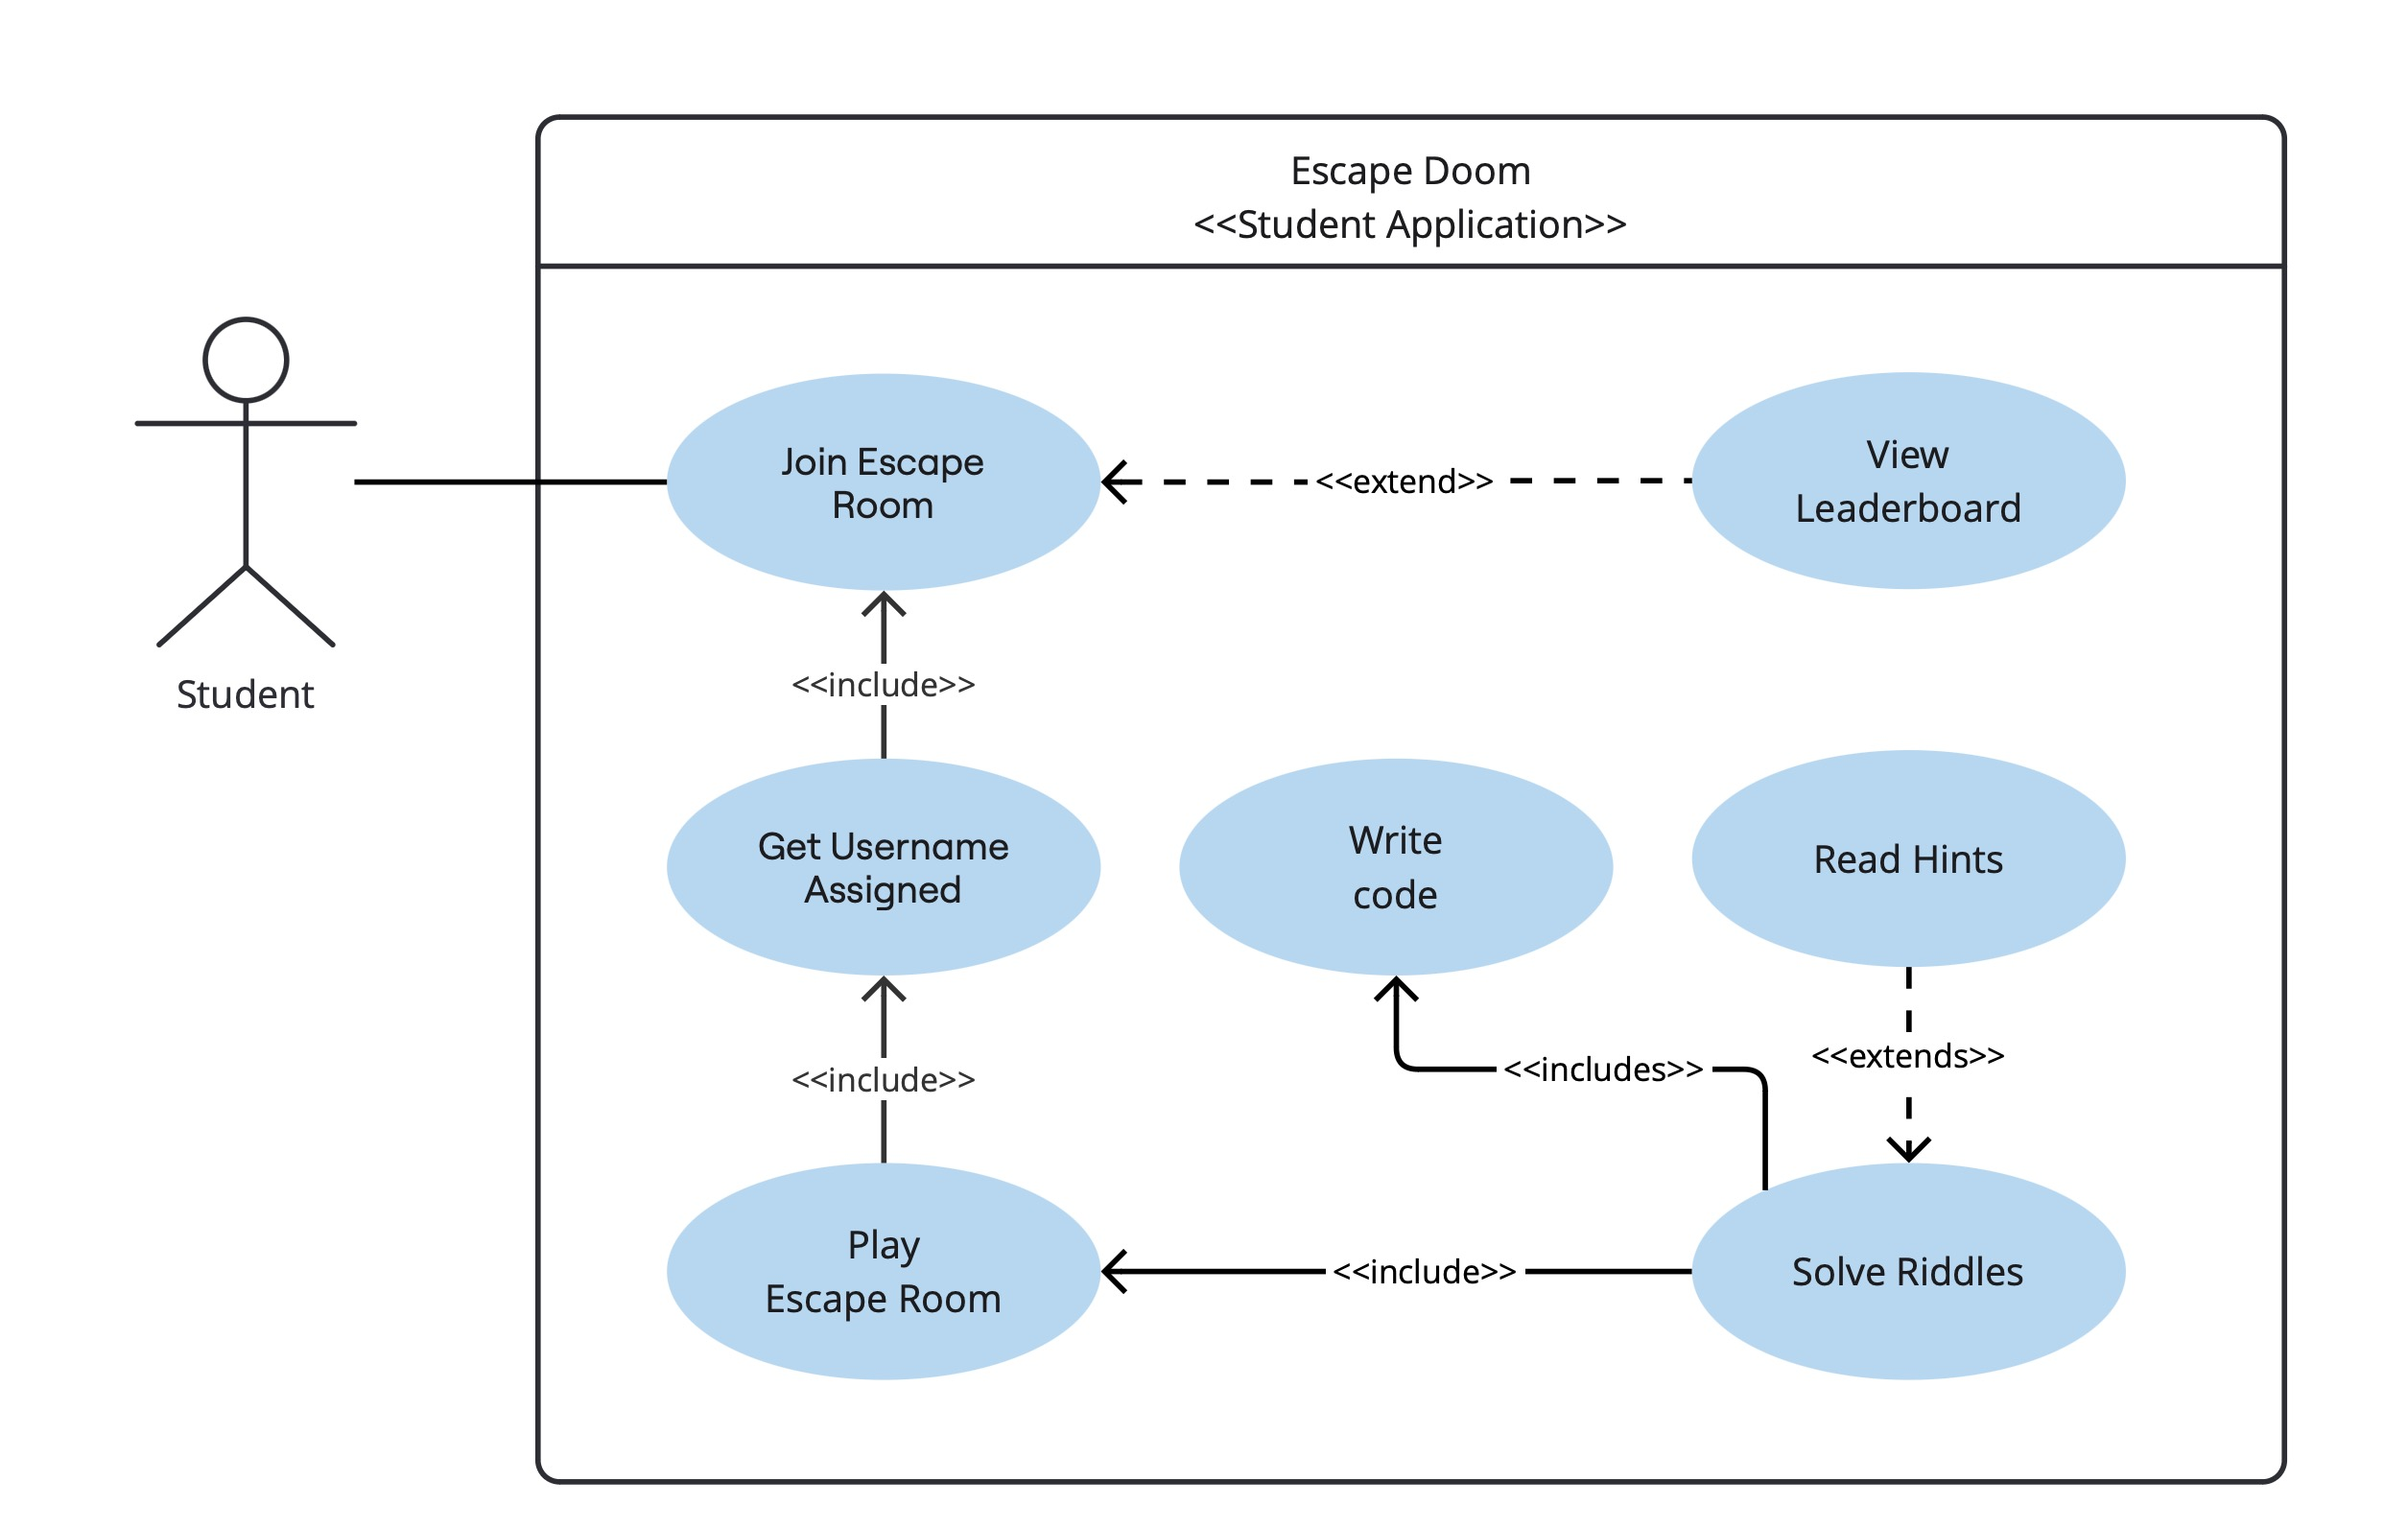
\includegraphics[width=\linewidth]{UC-02.png}
    \caption{UC02 - Student Application}
    \label{fig:uc-02}
\end{figure}
\newpage

\begin{figure}[h!]
    \centering
    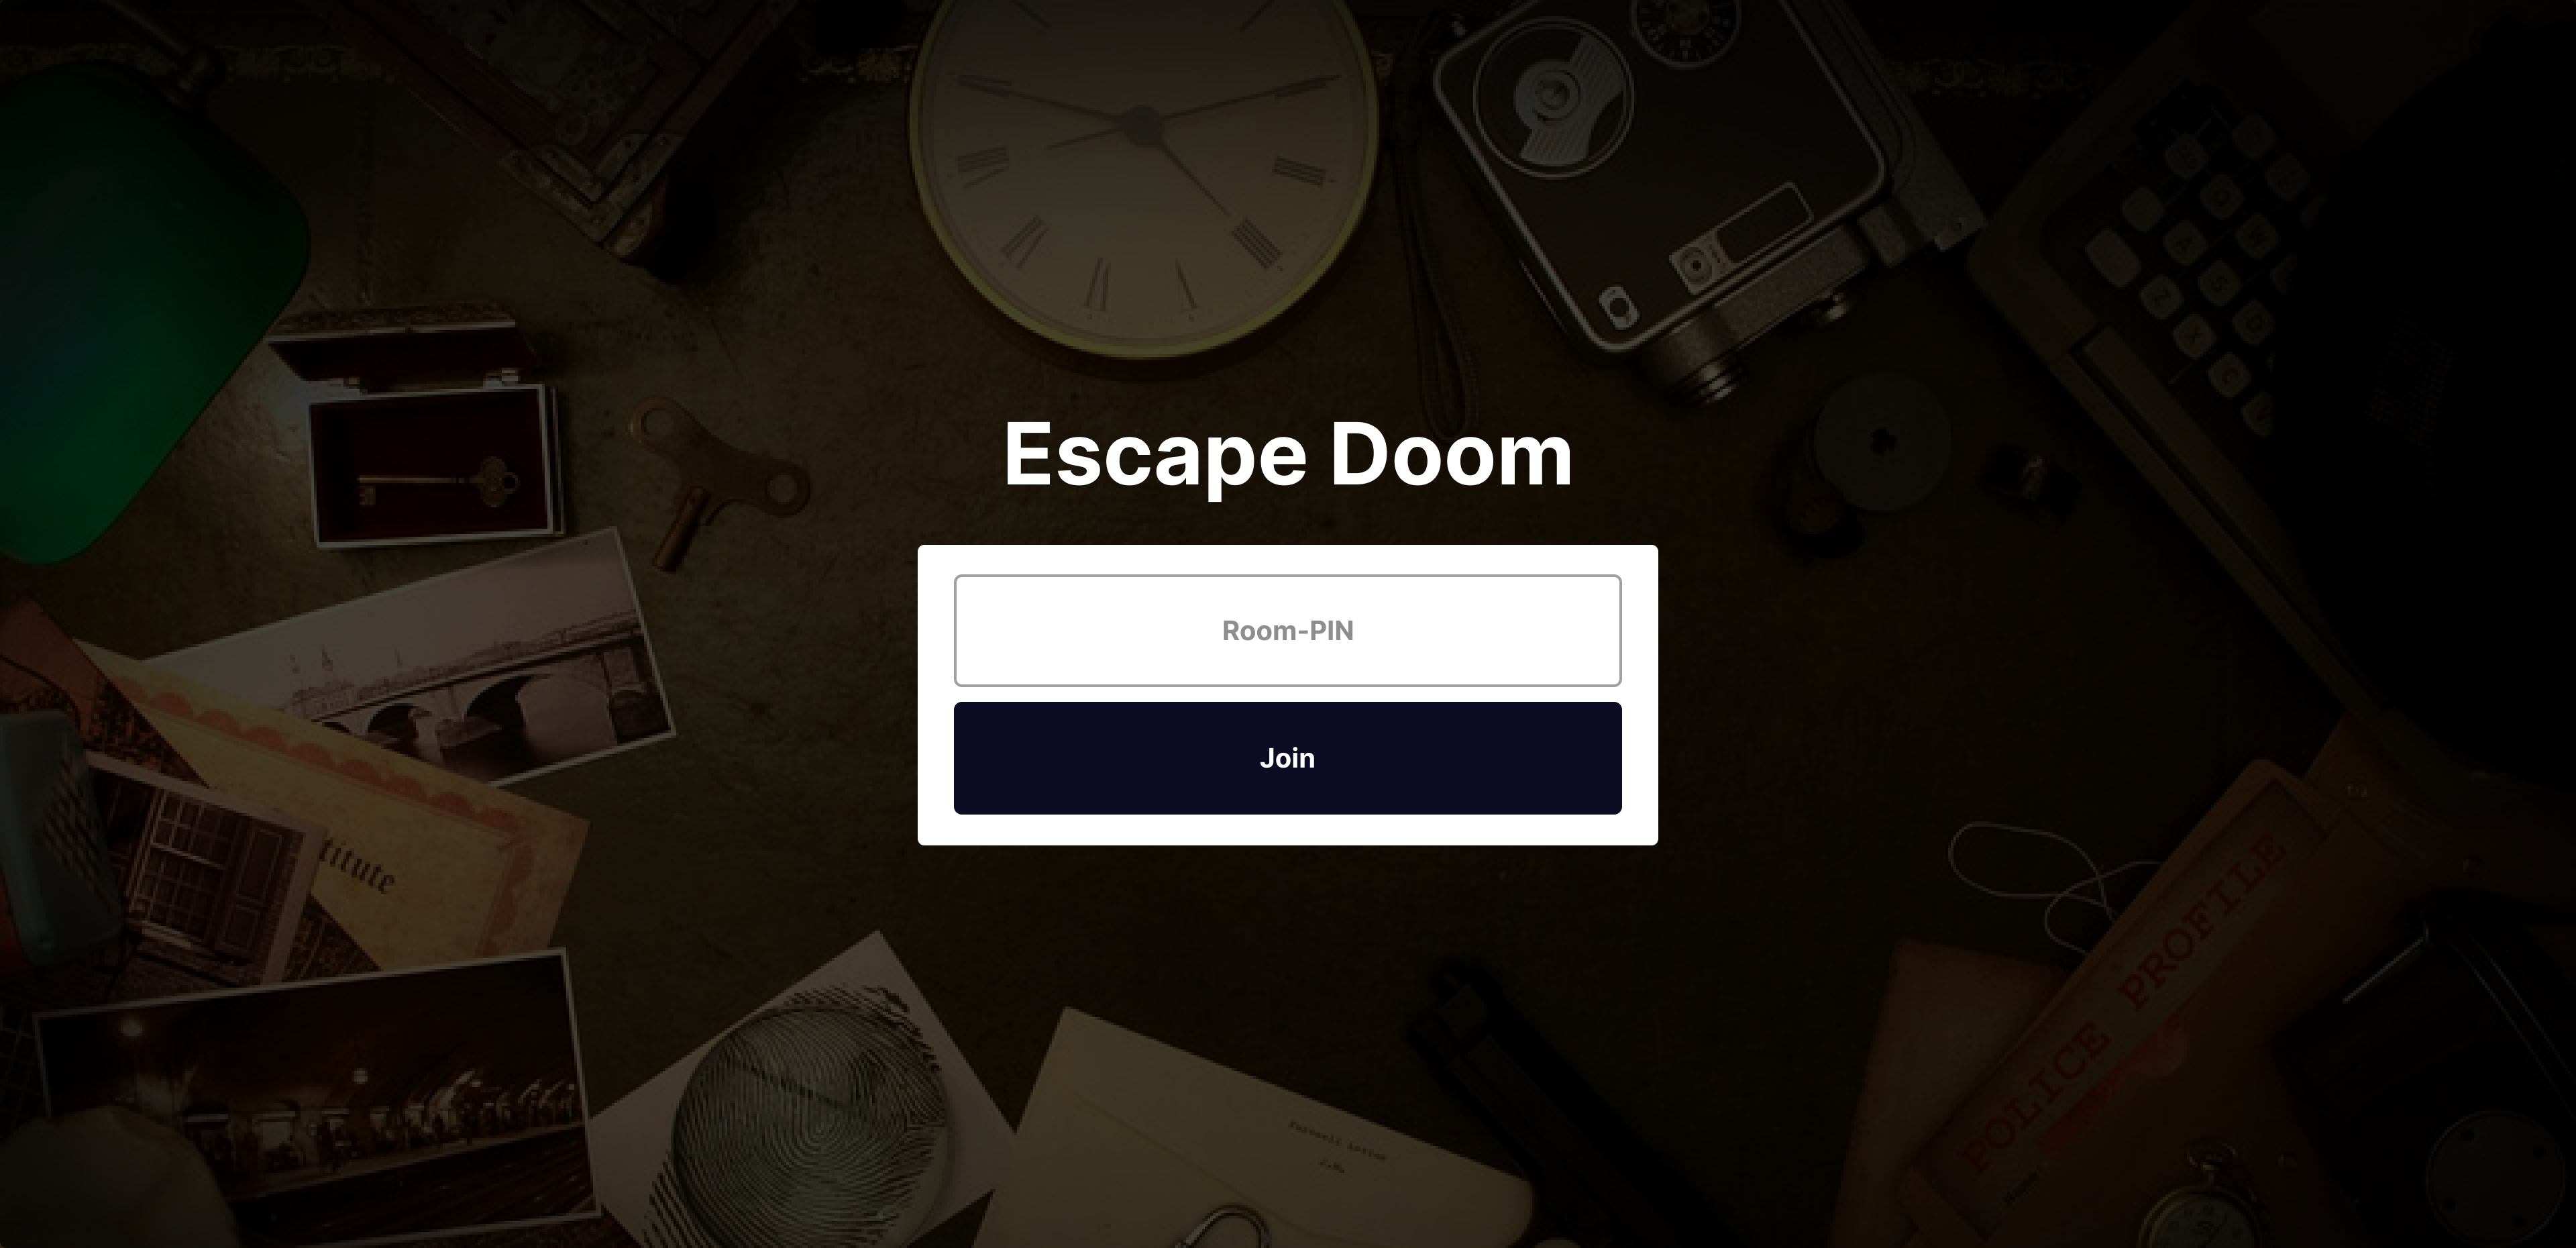
\includegraphics[width=\linewidth]{images/StudentJoin.png}
    \caption{Student Application Mockup}
    \label{fig:lector:portal}
\end{figure}